\documentclass{article}
\usepackage[italian]{babel}
\usepackage[T1]{fontenc}
\usepackage{graphicx}
\usepackage[utf8x]{inputenc}
\usepackage{amsmath}
\usepackage{amsthm}
\usepackage{hyperref}
\usepackage{caption}
\date{}
\author{Francesco Sacco Lorenzo Cavuoti}
\title{Caratteristiche porte logiche e semplici circuiti logici}

\begin{document}
\maketitle
\paragraph{0)}
	Lo scopo dell'esperienza è misurare le caratteristiche statiche e dinamiche delle porte NOT contenute nell’integrato SN74LS04 (HEX Inverter) e costruire semplici circuiti logici con le porte NAND.
	
\paragraph{1)}
	Si è montato il circuito in figura \ref{fig:circuito-1} e si è alimentato con $V_{CC}=4.7\pm0.2$ V usando solo un generatore. Successivamente si è fatta variare la resistenza del potenziometro e si è segnato $V_{in}$ e $V_{out}$ per ciascuna posizione del potenziometro, i dati sono riportati in tabella \ref{tab:124} e nel grafico in figura, le tensioni sono state misurate con i cursori dell'oscilloscopio.\newline

	\begin{minipage}{.6\linewidth}
		\centering
		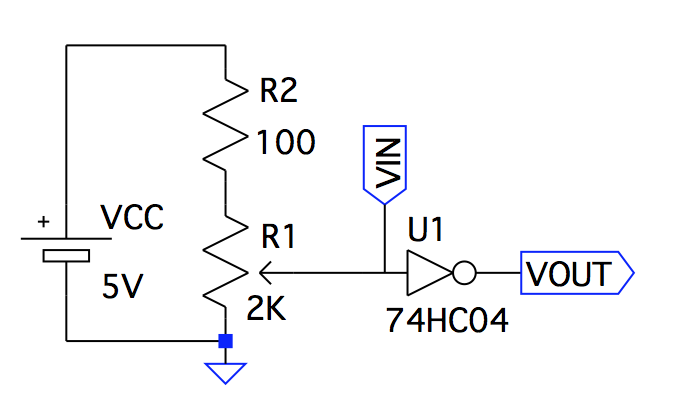
\includegraphics[width=\linewidth]{figure/circuito1}
		\captionof{figure}{Circuito 1}
		\label{fig:circuito-1}
	\end{minipage}
	\begin{minipage}{.4\linewidth}
		\begin{tabular}{cc}
\hline
	$V_{in}[V]$ & $V_{out}[V]$\\ 
\hline
	$4.6\pm0.2$ & $0.134\pm0.006$ \\
	$4.2\pm0.2$ & $0.134\pm0.006$ \\
	$3.2\pm0.1$ & $0.134\pm0.006$ \\
	$2.5\pm0.1$ & $0.134\pm0.006$ \\
	$1.84\pm0.09$ & $0.134\pm0.006$ \\
	$1.26\pm0.05$ & $0.134\pm0.006$ \\
	$1.16\pm0.05$ & $0.134\pm0.006$ \\
	$1.06\pm0.05$ & $2.5\pm0.1$ \\
	$1.04\pm0.05$ & $2.0\pm0.09$ \\
	$0.74\pm0.03$ & $4.1\pm0.2$ \\
	$0.34\pm0.01$ & $4.2\pm0.2$ \\
	$0.144\pm0.006$ & $4.2\pm0.2$ \\
\hline
\end{tabular}

		\label{tab:124}
	\end{minipage}\newline\newline

	Usando il potenziometro è stato possibile stimare i voltaggi VOH,VOL,VIH,VIL che si possono vedere nella tabella qui sotto.\newline
	Di conseguenza le bande d'incertezza misurate d'input è $0.418\pm0.007$, mentre quella di datasheet è $1.2 V$; la barra d'incertezza misurata d'output è $3.95\pm0.02$ e quella di datasheet è $3.2 V$.
	\begin{center}
		\begin{tabular}{ccc}
\hline
	Nome & Voltaggi misurati $[V]$ & Voltaggi datasheet $[V]$\\ 
\hline
	VOH & $4.1\pm0.2$ & 3.4 \\
	VOL & $0.134\pm0.006$ & 0.2 \\
	VIH & $1.16\pm0.05$ & >2 \\
	VIL & $0.74\pm0.03$ & <0.8 \\
\hline
\end{tabular}

	\end{center}

\paragraph{2)}
	Per il secondo punto abbiamo usato una resistenza di $3.31\pm0.03 k\Omega$, una frequenza di circa $1kHz$ e abbiamo mandato un'onda quadra di $5.0\pm0.2 V$.
	i tempi misurati sono $t_{PHL}=(7.2\pm0.8)ns$ (quello di datasheet è $10ns$), mentre $t_{PLH}=55\pm 1 ns$ (quello di datasheet è $25ns$).
	
\paragraph{3)}
	\subparagraph{a.}
	Si è montato il circuito in figura \ref{fig:NAND} dove i segnali A, B sono dati dallo DIP Switch a 4 interuttori con l'altro estremo collegato a massa.
	\subparagraph{b.}
	Per verificare velocemente la tabella di verità si è collegato un led all'uscita dei circuiti logici, cosi' da notare il passaggio di corrente senza dover misurare con il multimetro o l'oscilloscopio.
	
	\subparagraph{c.}
	\begin{description}
		\item[i.] Per costruire la porta AND (figura \ref{fig:AND}) si sono utilizzate 2 porte NAND. Prima si esegue A NAND B, successivamente si nega il segnale in uscita cosi' da ottenere A AND B
		\item[ii.] Per la porta OR (figura \ref{fig:OR}) si sono utilizzate 3 porte NAND, infatti sfruttando le leggi di De Morgan si ha: A OR B = (!A) NAND (!B) 
		\item[iii.] Per la porta XOR (figura \ref{fig:XOR}) si sono utilizzate 4 porte NAND,  il circuito è sempre stato ricavato dalle leggi di De Morgan
		\item[iv.] Per il sommatore ad un bit (figura \ref{fig:sommatore}) si sono utilizzate 6 porte NAND, anche se il circuito risulta abbastanza complicato in realtà questo è composto  da uno XOR, che da il valore del bit più significativo, e da un AND che da il valore del bit meno significativo. In fase di analisi ci siamo accorti che per il circuito bastavano 5 porte NAND, infatti A NAND B viene già fatto nello XOR e di conseguenza si può risparmiare una porta nel calcolo di A AND B; tuttavia questo porta il gate NAND1 ad avere 3 porte in uscita al posto di 2, mentre il tempo di propagazione resta teoricamente invariato rispetto al circuito precedente.\newline
	\end{description}

	\begin{minipage}{.45\linewidth}
		\centering
		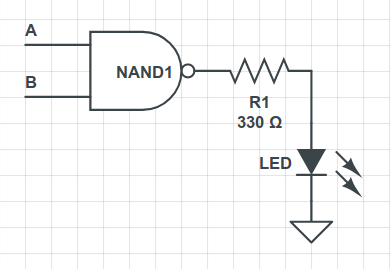
\includegraphics[width=\linewidth]{figure/NAND}
		\captionof{figure}{Schema circuitale NAND}
		\label{fig:NAND}
	\end{minipage}
	\begin{minipage}{.6\linewidth}
		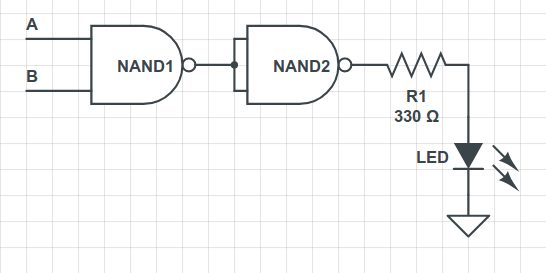
\includegraphics[width=\linewidth]{figure/AND}
		\captionof{figure}{Schema circuitale AND}
		\label{fig:AND}
	\end{minipage}\newline
	
	\begin{minipage}{.5\linewidth}
		\centering
		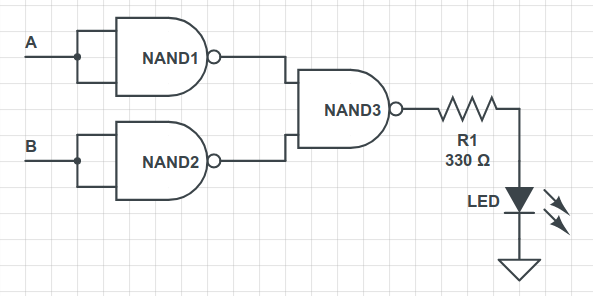
\includegraphics[width=\linewidth]{figure/OR}
		\captionof{figure}{Schema circuitale OR}
		\label{fig:OR}
	\end{minipage}
	\begin{minipage}{.55\linewidth}
		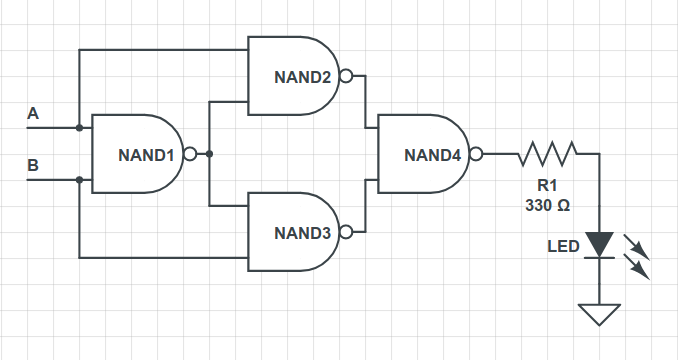
\includegraphics[width=\linewidth]{figure/XOR}
		\captionof{figure}{Schema circuitale XOR}
		\label{fig:XOR}
	\end{minipage}\newline
	
	\begin{figure}
		\centering
		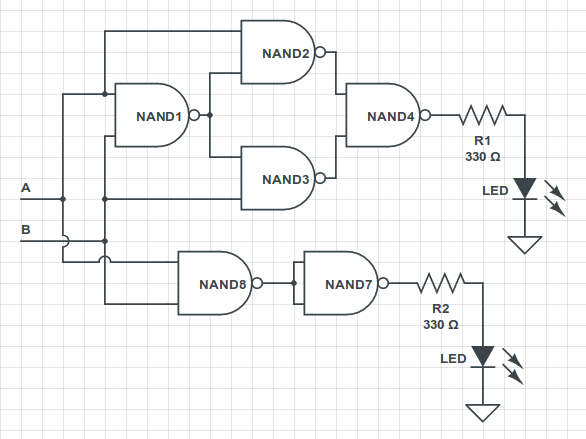
\includegraphics[width=\linewidth]{figure/Sommatore}
		\caption{Schema circuitale sommatore a un bit}
		\label{fig:sommatore}
	\end{figure}



\end{document}